\chapter{Introduction}\label{chap:introduction}

\todo{Rewrite intro}
Music has always been communicated in two ways: aural transmission, where music is played or performed and people can listen to it, and written transmission, where music is formalized in a document. These written formats come in many forms, one of which is western musical notation. These documents, mostly referred to as (music) scores, used to be handwritten, but were later printed on paper and can nowadays be found in digital format on computers, mostly as images or scans. Quite some effort has been taken to collect all of these digital scores and store them in central places or make them available to the public where possible. An example is the IMSLP library, where vast amounts of scores for classical music in the public domain are available. Collections such as these give rise to many opportunities, such as affordable scores and sheet music for musicians, or easy access to musical data for researchers. The formats in which these scores are stored do have their limitations however. When text is contained in PDF documents (or many other document forms for that matter), the text is recognized by the computer as text, meaning it can be searched, edited and reformatted. For music this is not the case. Scanned music scores are simply stored as images in PDF documents, meaning that none of the applications for text can be applied to these scores. This means that a lot of applications that the digital age provides cannot yet be applied to music scores and as such there is a huge gap for potential left open.

\section{Music notation}\label{sec:introduction-music-notation}
Music notation is the manner in which music is communicated in written form. The de facto standard for this since the seventeeth century has been Common Western Music Notation (CWMN), of which the general principles are shared by almost all music that is written since then. CWMN consists of one or more music parts, which are depicted from left to right, synchronized in time. The music is divided up into measures, which provide logical divisions and keep track of the current position in the music while playing. These measures are seperated by barlines. Since measures are used to track the position of music in time, the different parts all have the same amount of measures, synchronized in time. To make sure these parts fit on pages, they are broken up at barlines and placed under each other on the page, or on the next page if there is no more space on the page left. This pattern resumes till the end of the piece. Each such section that spans a page's width is called a system, which consists of a set a staffs, generally one for each part, all divided into synchronized measures. We call the collection of measures that overlap at a given point in time a system measure, to differentiate them from the individual measures. It can be customary to leave out staffs of a system if that part has nothing to play for the duration of that system, causing difference in the number of staffs between systems. In Figure \ref{fig:page-structure} examples of all these elements of CWMN are shown. In first of the two systems is highlighted in yellow, the second staff of the first system is highlighted in red, the first system measure is highlighted in green and the first measure of the third part is highlighted in blue. When counting, it also becomes clear that the first system has one staff more than the second system, to save space on the page.

When going to a smaller level, we touch upon the contents of the individual measures. The vertical placement of notes indicate their pitch, together with the clefs and accidentals that might occur on the page or in the measure. Their horizontal relation to each other, as well as the type of note, flags, and rests, indicate the rhythm in which the notes need to be played. Those at least are the very basic principles, ignoring a vast amount of details. One special case that is worth noting is the empty measure, which consists entirely of a single, full-measure rest without any notes. This indicates that in this measure the instrument has no role to play, examples can be seen in figure \ref{fig:page-structure}, e.g. the last four measures of the top three staffs. 

\begin{figure}
    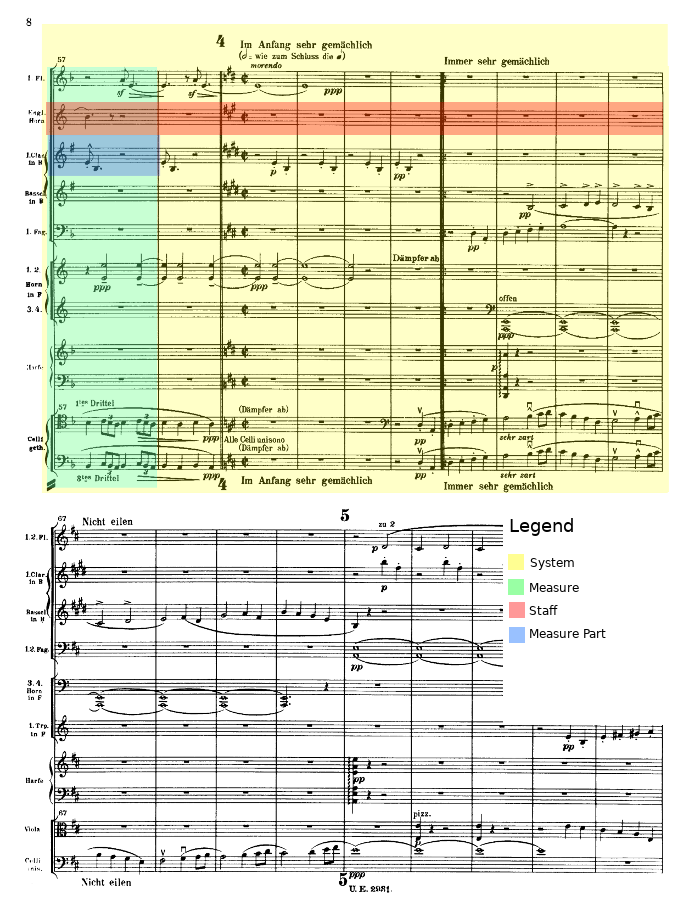
\includegraphics[width=\textwidth]{images/score-structure.png}
    \centering
    \caption{Example structure of a page of music}
    \label{fig:page-structure}
\end{figure}

\section{Introduction into Optical Music Recognition}\label{sec:introduction-OMR}
By digitizing the contents of a music score, the information contained in it can be processed by a computer. This opens up a large amount of possibilities for various target audiences. First of all the field of musicology can benefit greatly from this, since digital scores are often not availble. Cultural heritage can be safeguarded through digital scores, since large amounts of historical significant collections of music are currently only available on paper. Musicians can be equiped with a ``digital music stand'', where the music score can be easily adapted to account for readability issues, or error corrections and annotations can be easily made and shared with other musicians. Furthermore there is the obvious advantage of compiling large databases of digital information, creating possibilities for search and browsing, which are widely available for textual data, and further applications such as melody retrieval and similarity studies, just to name a few.

The digitizing process, or transcribing, is still relatively often done manually by experts. Several music notation applications can be found nowadays, which make their workflow more efficient. Examples of these applications are Sibelius \footnote{https://www.avid.com/sibelius}, MuseScore \footnote{https://musescore.org/} and Finale \footnote{https://www.finalemusic.com/}, in which users can input music either by keyboard and mouse, or by using a MIDI keyboard. The large drawback of these systems is that inputting music is time-consuming and takes experience, and is therefore expensive. Automatic transcription of music scores could therefore dramatically improve this process, and this is what the field of Optical Music Recognition, or OMR, is researching.

Automating transcription is unfortunately not an easy task. There are a lot of parallels to be drawn with the field of Optical Character Recognition, which focusses on transcribing written text. However, where most OCR tasks are considered to be solved, this does not hold for OMR. There are several reasons for this. First of all, where OCR is generally a one dimensional problem where text is vertically evenly spaced out, OMR is a two dimensional problem, where time and frequency make up the horizontal and vertical axis of sheet music, respectively \citep{Bainbridge2001, Byrd2015}. This can result in influence between symbols that are spaced out far across the page, such as a clef at the start of a page, which indicated what frequency the written notes entail, or accidentals that span a measure or even an entire page's width. Additionally, in music different symbols can be stacked on top of one another to signify multi-tones or chords, or can be connected horizontally to one another. Stacked or connected notes can also be translated both horizontally and vertically relative to each other, meaning the connection can become stretched or tilted, see \citep{Bainbridge2001} for some examples. Besides, these translations and connections can often be done in different ways, or they can be purposefully left out. Decisions on if and how these tranformations are used often depend on preferences of the musician, or on larger contextual requirements, such as horizontal spacing to accommodate space for measures that are played at the same time. Furthermore there are symbols that are relatively small in comparison to the notes, but have significant meaning, such as dots, dashes and accents. There is also a large imbalance in the frequency in which symbols occur, increasing the likelihood of false positives when classifying these symbols \citep{Chen2016b}. The collection of musical symbols is also not entirely fixed, and new symbols are added regularly \citep{Fujinaga1996} and on top of all this, scanned music notation that is subject to OMR is often blurry, noisy or fragmented. All of these difficulties make it impossible for simple systems to accurately transcribe music scores.

The OMR field has been active for over 50 years now, starting with Pruslin in 1966 \citep{Pruslin1992}. Since then, a number of different approaches have been tried, which ultimately led to a generally agreed upon pipeline in which the OMR task could be subdivided into smaller subtasks. This pipeline was first coined by Bainbridge and Bell \citep{Bainbridge2001} and was later elaborated on by Rebelo et al. \citep{Rebelo2012} in a vast literature review. Both papers indicate that the vast majority of research up to that point could be segmented into the various stages of this pipeline, and in fact a lot of research from that point on falls into place when considering this framework. Although research following this pipeline progresses, most of it suffers from a lack of fixed evaluation metrics. Divising suitable error metrics in OMR research is a hard problem, and shared datasets are hard to come by, making it difficult to compare different solutions \citep{Bellini2007, Byrd2015}. There have been deviations though, since not all stages are equally easily solvable. With the increasing research and application of deep learning, attempts at full-pipeline and end-to-end OMR have been started to occur as well \citep{CalvoZaragoza2017, Pacha2019, Wel2017}. The preliminary results show promise, but the research effort is scoped very tightly, making it so that a lot of work needs to be done before these approaches can be considered generally applicable. This is also hampered by the main struggle of deep learning; the lack of sufficient data. Some datasets have been compiled, mainly for object classifications, but it is hard to conceive that these will be sufficient for reliable classification given the large amount of variability that these objects can occur in due to differences in handwriting, typesetting and deformations in printing and scanning.

Due to all of these problems, current workflows tend to pipe the result of an OMR system into a music notation application for human error correction. This process of human correction at the end is still very expensive, Bellini et al. \citep{Bellini2007} claim that even a recognition rate of 90\% does not make an OMR system attractive to music copyists. Attempts at human-aided OMR are therefore made, where the focus lies on human feedback in several stages of the pipeline instead of at the end of the process. The hope is that this will either reduce the total time required of expert users or make non-expert user feedback an option to improve the performance of such an OMR system in comparison to fully automated versions. Examples of such research are MacMillan et al. \citep{Macmillan2002}, who have developed Gamera, an ease-to-use scripting environment for OMR, Chen et al. \citep{Chen2016, Chen2016b}, who have been developing an adapted OMR system called Ceres that takes human feedback into account, and Burghardt and Spanner \citep{Burghardt2017}, who developed Allegro which takes a more user-centered approach and provides an easy framework for users to transcribe the contents of simple handwritten scores.

\section{TROMPA}\label{sec:introduction-TROMPA}
Towards Richer Online Music Public-domain Archives, or TROMPA, is an international organization of scientists, scholars and musicians that push towards the goal of making more applications available to the music domain and increase engagement with classical music and music scores \citep{TROMPAwebpage}. One of their main research themes is called ``Scanned score analysis'' and focusses on improving OMR and bringing together different techniques to make large scale transcription of music scores feasible, so that those transcriptions can be used in a variety of other research themes. Within this research theme, work is being done on human-aided OMR through crowd computing, in which a large userbase is asked to interact with the results of an OMR system and through that correct and check the results of the system.

\issue{Await TROMPA deliverable}

Viewing these results, one of the issues that arises when dealing with large music works like this is the repetitiveness of correcting and checking measures of the music score. Especially in large ensemble works, it occurs frequently that several instruments or instrument groups don't play continuously, but instead have parts of the piece where there is a gap in their score. Since these instrument groups still need to be aligned with the rest of the ensemble in the music score, these parts are indicated by empty measures. Over the different instrument groups, the total of these empty measures can add up quickly, which raises the question whether this characteristic can be utilized to improve the workflow of this human-aided OMR system, and perhaps reduce the work that has to be performed by users.

\section{Problem statement}\label{sec:introduction-problem-statement}
This leads to the main goal of this thesis. We want to investigate whether the work needed for this OMR task can be made easier by means of finding similarities in the music scores on the measure level. If it is indeed possible to find such similarities, and we can separate these similar measures with reasonable accuracy from the remainder of the score, data that is collected on these measures, be it through automated transcription or human input, could be shared across similar measures. This also means that the benefits of such a system would not be limited to the TROMPA project, but could be applied in a wider OMR context. These similarities will be studied on PDF documents that contain the scores, since those documents are the main targets for (automatic) transcription in the TROMPA project. The scope of music is defined as follows:

\begin{itemize}
    \item We focus on ensemble music, that is, music written for ensembles of musicians. These ensembles can range from small chamber music ensembles, which usually consist of two to eight musicians, to full-sized symphony orchestras. This scope is a logical one given the goal this thesis is persuing, since similarities in music, such as empty measures, are more likely to occur in larger ensembles. Music written for individual permormers will most likely contain very little empty measures.
    \item We focus on music scores that are available in typeset fonts, since the vast majoriy of these ensemble works can be found as typeset in public domain collections such as the Petrucci Music Library (IMSLP \citep{IMSLP}).
\end{itemize}

To be able to find these similarities, we first need to be able to accurately find the measures that are found in a given score. Therefore a preliminary step needs to be taken which can segment the music score in PDF format into its individual measures. This is the first part of our research goal, after which we can focus on the similarity study.

\section{Research questions}\label{sec:introduction-research-questions}
Now that we have defined the problem, we define the following main research question:

\begin{quote}
    {\itshape \textbf{RQ}: How can we find similarities in music scores on the measure level?}
\end{quote}

\noindent To structure this further, we provide the following subquestions:

\begin{quote}
    {\itshape \textbf{SQ1}: What previous work has been done on measure detecting and similarity finding and how can we build upon this?}

    {\itshape \textbf{SQ2}: What data is available which can be used to design and evaluate these systems?}

    {\itshape \textbf{SQ3}: How can we reliably detect the measures in a music score?}

    {\itshape \textbf{SQ4}: How can we find similarities between detected measures?}
\end{quote}

\section{Main contributions}\label{sec:introduction-contributions}

\section{Outline}\label{sec:introduction-outline}
